% Extrait du rapport general du mini-projet GANs et diffusion.
% Contribution : sections "Dataset" et "Partie 1 - Generation avec un GAN".
% A integrer dans le rapport general (4 a 8 pages) une fois les autres parties redigees.

\section{Dataset --- Fashion-MNIST}
\label{sec:dataset}

\subsection{Description et justification}

Le dataset utilise pour ce mini-projet est \textbf{Fashion-MNIST}~\cite{xiao2017fashion}, propose par Zalando comme alternative directe a MNIST. Il contient 70~000 images en niveaux de gris, de resolution $28 \times 28$ pixels, reparties en 10 classes vestimentaires : T-shirt, Pantalon, Pull, Robe, Manteau, Sandale, Chemise, Sneaker, Sac et Bottine. Le split standard est de 60~000 images d'entrainement et 10~000 images de test.

Ce choix est pertinent pour un projet de comparaison GAN versus diffusion pour trois raisons :

\begin{itemize}
    \item \textbf{Cout de calcul modere.} La resolution $28 \times 28$ permet d'entrainer un GAN complet sur GPU grand public en moins de 5 minutes, ce qui rend les iterations experimentales realistes dans le cadre d'un mini-projet.
    \item \textbf{Structure plus riche que MNIST chiffres.} Les classes vestimentaires presentent des silhouettes plus variees et des chevauchements visuels (T-shirt vs Chemise vs Pull, Sneaker vs Sandale vs Bottine), ce qui revele les vrais comportements pathologiques d'un modele generatif --- mode collapse, hybridation de classes, perte de details fins.
    \item \textbf{Equilibre parfait.} 6~000 images de train et 1~000 de test par classe (figure~\ref{fig:fashion-distribution}). Aucune ponderation n'est necessaire et toute disparite observee dans la generation est imputable au modele, pas a un biais d'echantillonnage.
\end{itemize}

\begin{figure}[h]
    \centering
    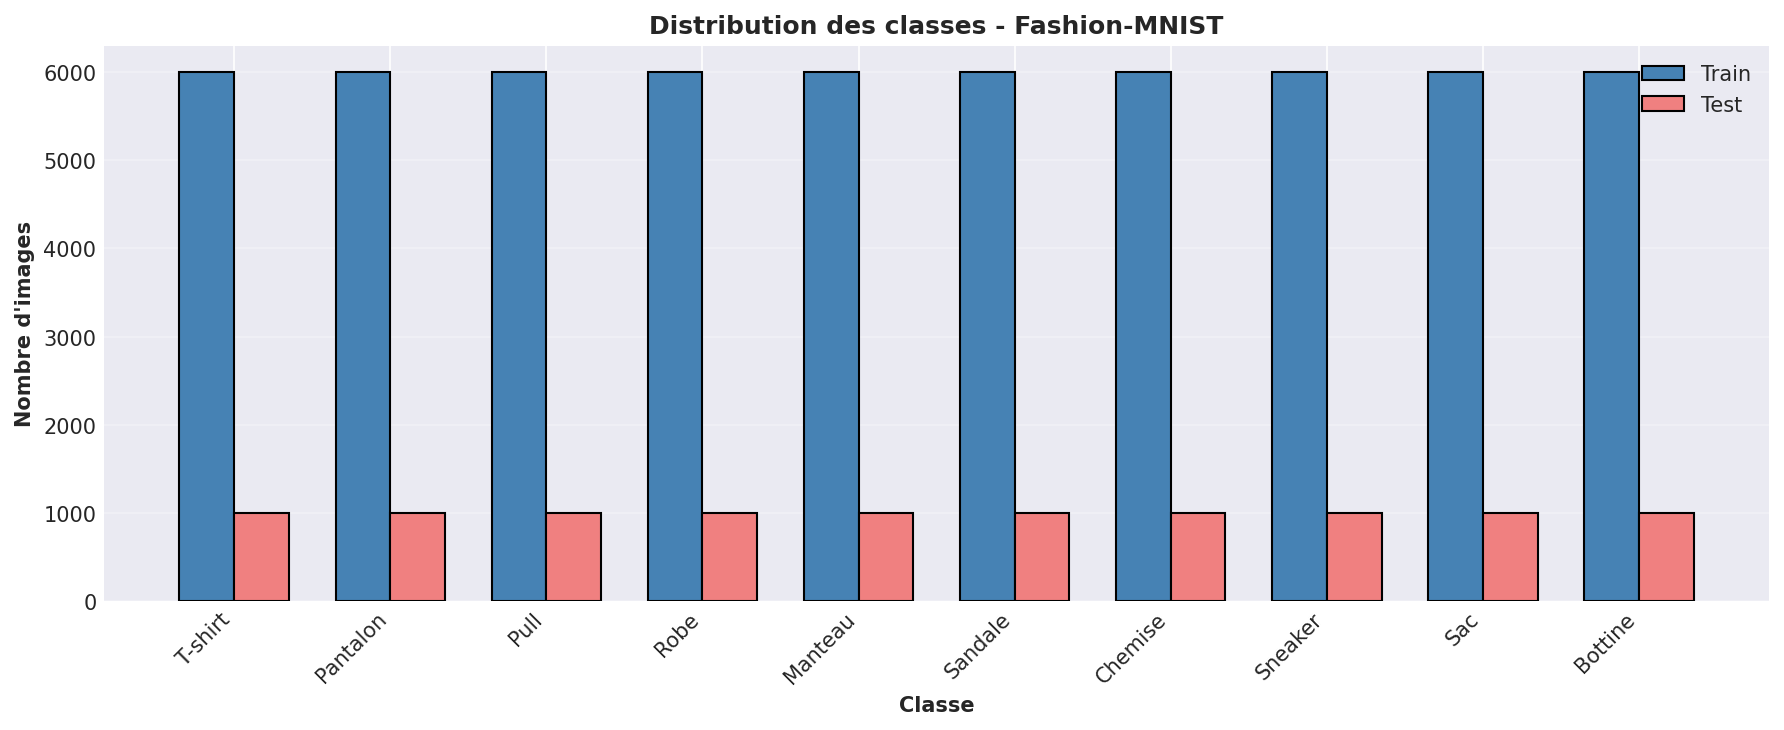
\includegraphics[width=0.95\linewidth]{02_distribution_classes.png}
    \caption{Distribution des classes Fashion-MNIST. Le dataset est parfaitement equilibre.}
    \label{fig:fashion-distribution}
\end{figure}

\subsection{Pretraitement}

Les images sont chargees via \texttt{torchvision.datasets.FashionMNIST} et normalisees dans l'intervalle $[-1, 1]$ par la transformation :
\[
    x' = \frac{x - 0{,}5}{0{,}5}
\]
Ce choix est dicte par la sortie \texttt{Tanh} du generateur GAN, qui produit elle aussi des valeurs dans $[-1, 1]$. Une normalisation $[0, 1]$ aurait force a utiliser une \texttt{Sigmoid} en sortie du generateur, notoirement moins stable a l'entrainement adversarial. La verification empirique sur un batch retourne : min $= -1{,}0000$, max $= 1{,}0000$, moyenne $\approx -0{,}43$, ecart-type $\approx 0{,}70$. La moyenne negative reflete simplement la predominance des pixels noirs (fond) dans les images.

\begin{figure}[h]
    \centering
    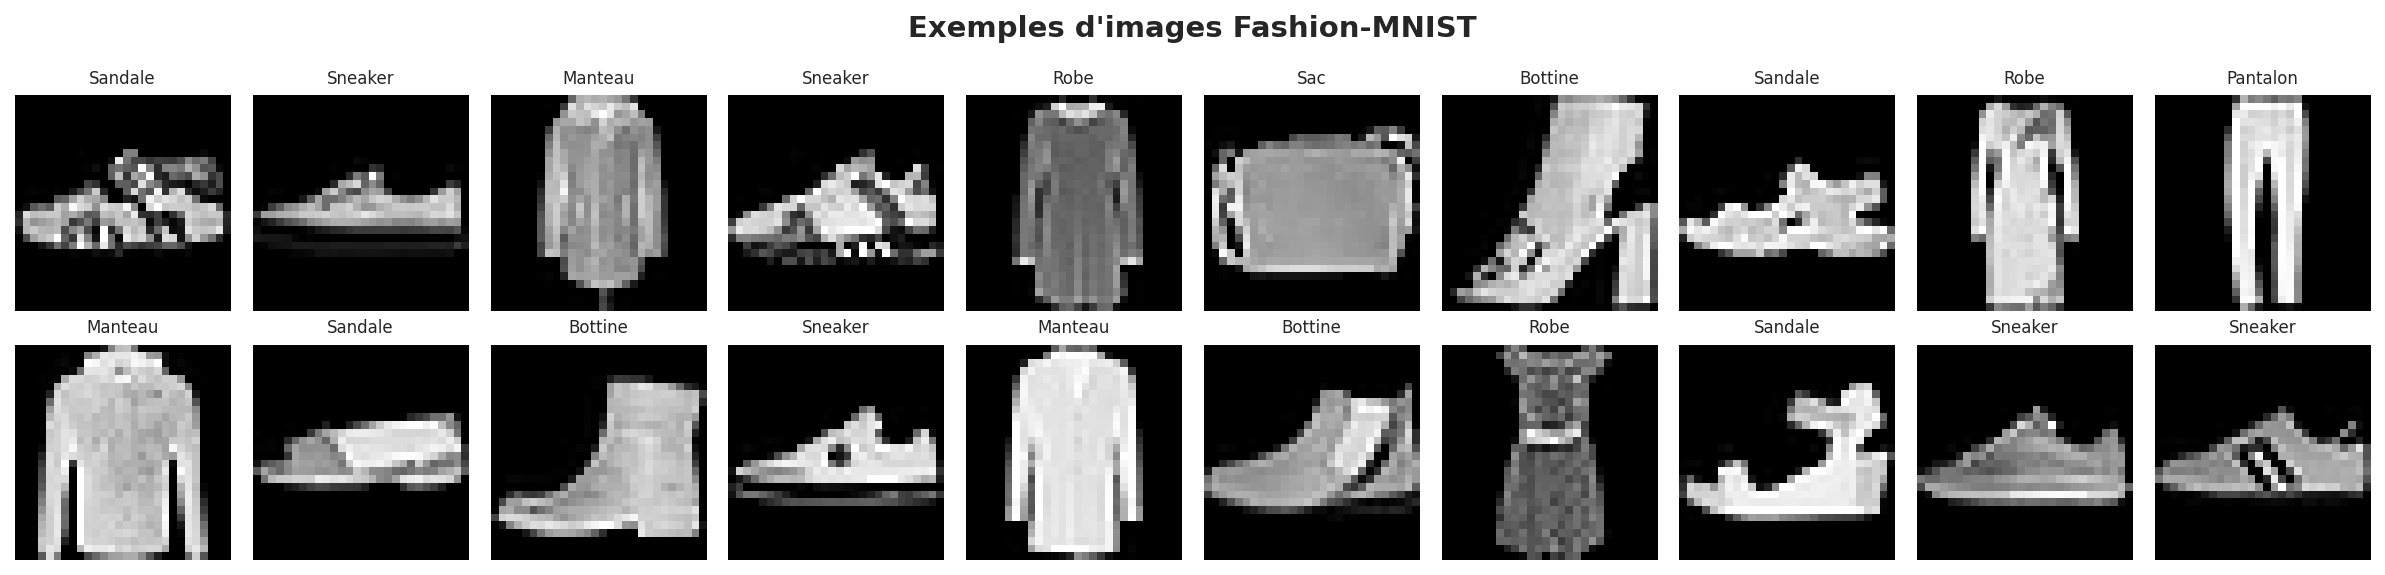
\includegraphics[width=0.95\linewidth]{01_exemples_images.png}
    \caption{Echantillon de 20 images Fashion-MNIST apres normalisation, denormalisees pour l'affichage.}
    \label{fig:fashion-samples}
\end{figure}

\subsection{Difficultes anticipees pour la generation}

L'inspection des echantillons (figure~\ref{fig:fashion-samples}) revele plusieurs caracteristiques qui poseront probleme aux modeles generatifs :

\begin{itemize}
    \item \textbf{Similarite inter-classes.} T-shirt, Pull, Chemise et Manteau partagent une silhouette de base (corps + manches). Un modele non conditionne aura tendance a produire des images intermediaires non identifiables.
    \item \textbf{Details fins sous-representes.} A $28 \times 28$ en niveaux de gris, les lacets, sangles, boutons, cols et motifs imprimes sont coderes par tres peu de pixels et sont les premiers a etre lisses par le generateur.
    \item \textbf{Multi-modalite intra-classe.} La meme classe ``Chaussure'' contient des vues de cote, des sandales plates, des bottes hautes, des sneakers : un generateur doit capturer plusieurs sous-modes, ce qui favorise le mode collapse.
    \item \textbf{Absence de couleur.} Le modele doit s'appuyer exclusivement sur la forme et le contraste pour distinguer les classes.
\end{itemize}

Ces difficultes serviront de grille de lecture pour evaluer les modeles dans la suite du rapport.

\section{Partie 1 --- Generation avec un GAN}
\label{sec:gan}

\subsection{Architecture DCGAN}

Nous avons retenu une architecture \textbf{DCGAN}~\cite{radford2015dcgan} adaptee au format $28 \times 28$ plutot qu'un GAN purement dense ou une variante plus complexe (WGAN-GP, StyleGAN). Le DCGAN est devenu la baseline canonique pour la generation d'images naturelles : il combine convolutions transposees avec strides, \texttt{BatchNorm}, \texttt{ReLU}/\texttt{LeakyReLU} et \texttt{Tanh} de sortie, recettes qui font converger l'entrainement de maniere fiable sans regularisation supplementaire.

\paragraph{Generateur} ($\approx$ 4{,}88 M parametres). Projection dense du vecteur latent $z \in \mathbb{R}^{100}$ vers un tenseur $7 \times 7 \times 256$, puis deux \texttt{ConvTranspose2d} (stride 2, kernel 4) qui doublent la resolution a chaque etape : $7 \to 14 \to 28$. Chaque couche intermediaire est suivie de \texttt{BatchNorm2d} + \texttt{ReLU}. La sortie est lissee par une \texttt{Conv2d} $3 \times 3$ suivie d'une \texttt{Tanh}.

\paragraph{Discriminateur} ($\approx$ 1{,}07 M parametres). Trois \texttt{Conv2d} avec strides ($28 \to 14 \to 7 \to 4$), \texttt{LeakyReLU(0.2)} et \texttt{BatchNorm2d} entre couches, suivies d'une projection dense vers un logit scalaire. Nous utilisons \texttt{BCEWithLogitsLoss} plutot que \texttt{Sigmoid + BCELoss}, plus robuste numeriquement lorsque les logits deviennent extremes.

\paragraph{Choix de la dimension latente.} \texttt{latent\_dim = 100}, valeur standard du papier DCGAN. Une dimension inferieure (16--32) limite la diversite des images generees, une dimension superieure (256+) n'apporte pas de gain mesurable sur ce dataset et complique l'optimisation.

\subsection{Hyperparametres d'entrainement}

\begin{table}[h]
    \centering
    \small
    \begin{tabular}{ll}
        \toprule
        \textbf{Parametre} & \textbf{Valeur} \\
        \midrule
        Dimension latente $z$ & 100 \\
        Batch size & 128 \\
        Nombre d'epochs & 50 \\
        Optimiseur & Adam ($\beta_1 = 0{,}5$, $\beta_2 = 0{,}999$) \\
        Learning rate G et D & $2 \times 10^{-4}$ \\
        Loss & \texttt{BCEWithLogitsLoss} (objectif non saturant) \\
        Initialisation & $\mathcal{N}(0, 0{,}02)$ pour Conv et Linear \\
        Seed globale & 42 \\
        \bottomrule
    \end{tabular}
    \caption{Hyperparametres retenus pour le DCGAN.}
    \label{tab:gan-hp}
\end{table}

La boucle d'entrainement alterne une mise a jour du discriminateur sur \texttt{BCE($D$(reel), 1) + BCE($D$(faux), 0)} puis une mise a jour du generateur sur \texttt{BCE($D$(faux), 1)} (formulation non saturante de Goodfellow). En fin de chaque epoch, on enregistre un snapshot de 16 images generees a partir d'un \textbf{bruit fixe}, ce qui permet de visualiser la convergence du generateur sur les memes points latents au fil de l'entrainement (figure~\ref{fig:gan-evolution}). Sans cette astuce, on melange l'effet de l'apprentissage et l'effet du sampling, et la lecture devient ambigue.

\subsection{Analyse des courbes de loss}

\begin{figure}[h]
    \centering
    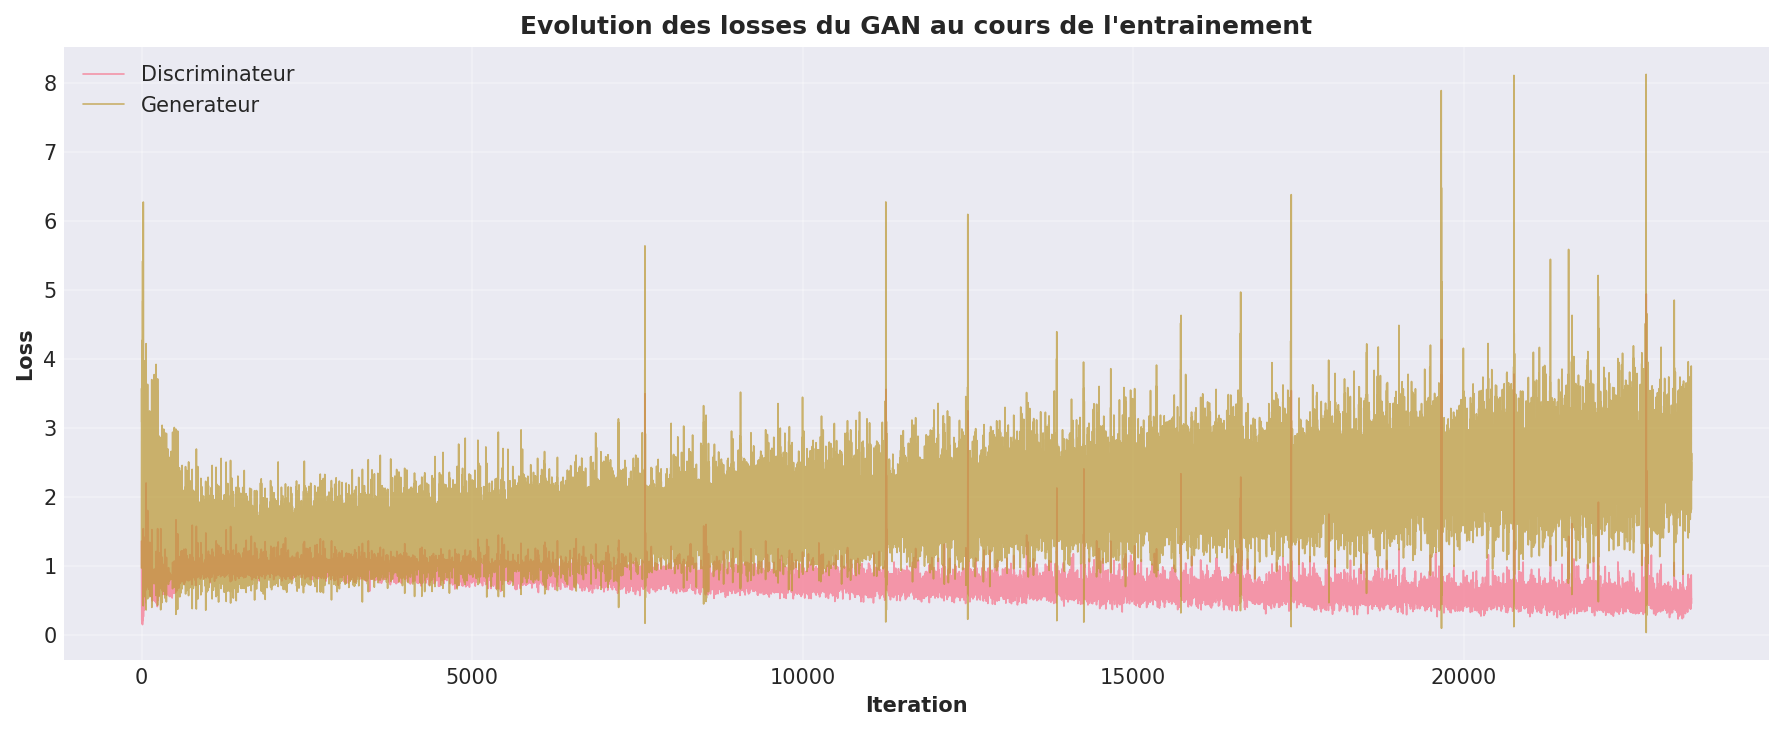
\includegraphics[width=\linewidth]{03_gan_losses.png}
    \caption{Evolution des losses du generateur et du discriminateur sur les 50 epochs ($\approx$ 23~000 iterations).}
    \label{fig:gan-losses}
\end{figure}

La figure~\ref{fig:gan-losses} montre un patron classique : la \texttt{D\_loss} se stabilise dans la zone 0{,}5--1{,}0 (a comparer a l'optimum theorique $2\ln 2 \approx 1{,}39$), tandis que la \texttt{G\_loss} \emph{derive} progressivement vers le haut, de $\approx 2$ en debut a $\approx 3$--$4$ en fin d'entrainement, avec des pics ponctuels jusqu'a 8. Cette derive indique que le discriminateur prend l'avantage : le generateur reste capable de tromper $D$ la majorite du temps mais avec une marge qui se reduit.

Cette observation conduit a une lecon centrale du projet : \textbf{les losses GAN ne sont pas un proxy direct de la qualite visuelle}. Une \texttt{D\_loss} qui chuterait vers zero serait au contraire un mauvais signal --- gradient eteint pour $G$ --- et une \texttt{G\_loss} qui s'effondrerait brutalement traduirait souvent un mode collapse. Les losses servent surtout a detecter les pathologies, l'evaluation reelle se fait visuellement ou via des metriques specifiques (FID, IS).

\subsection{Resultats visuels}

\begin{figure}[h]
    \centering
    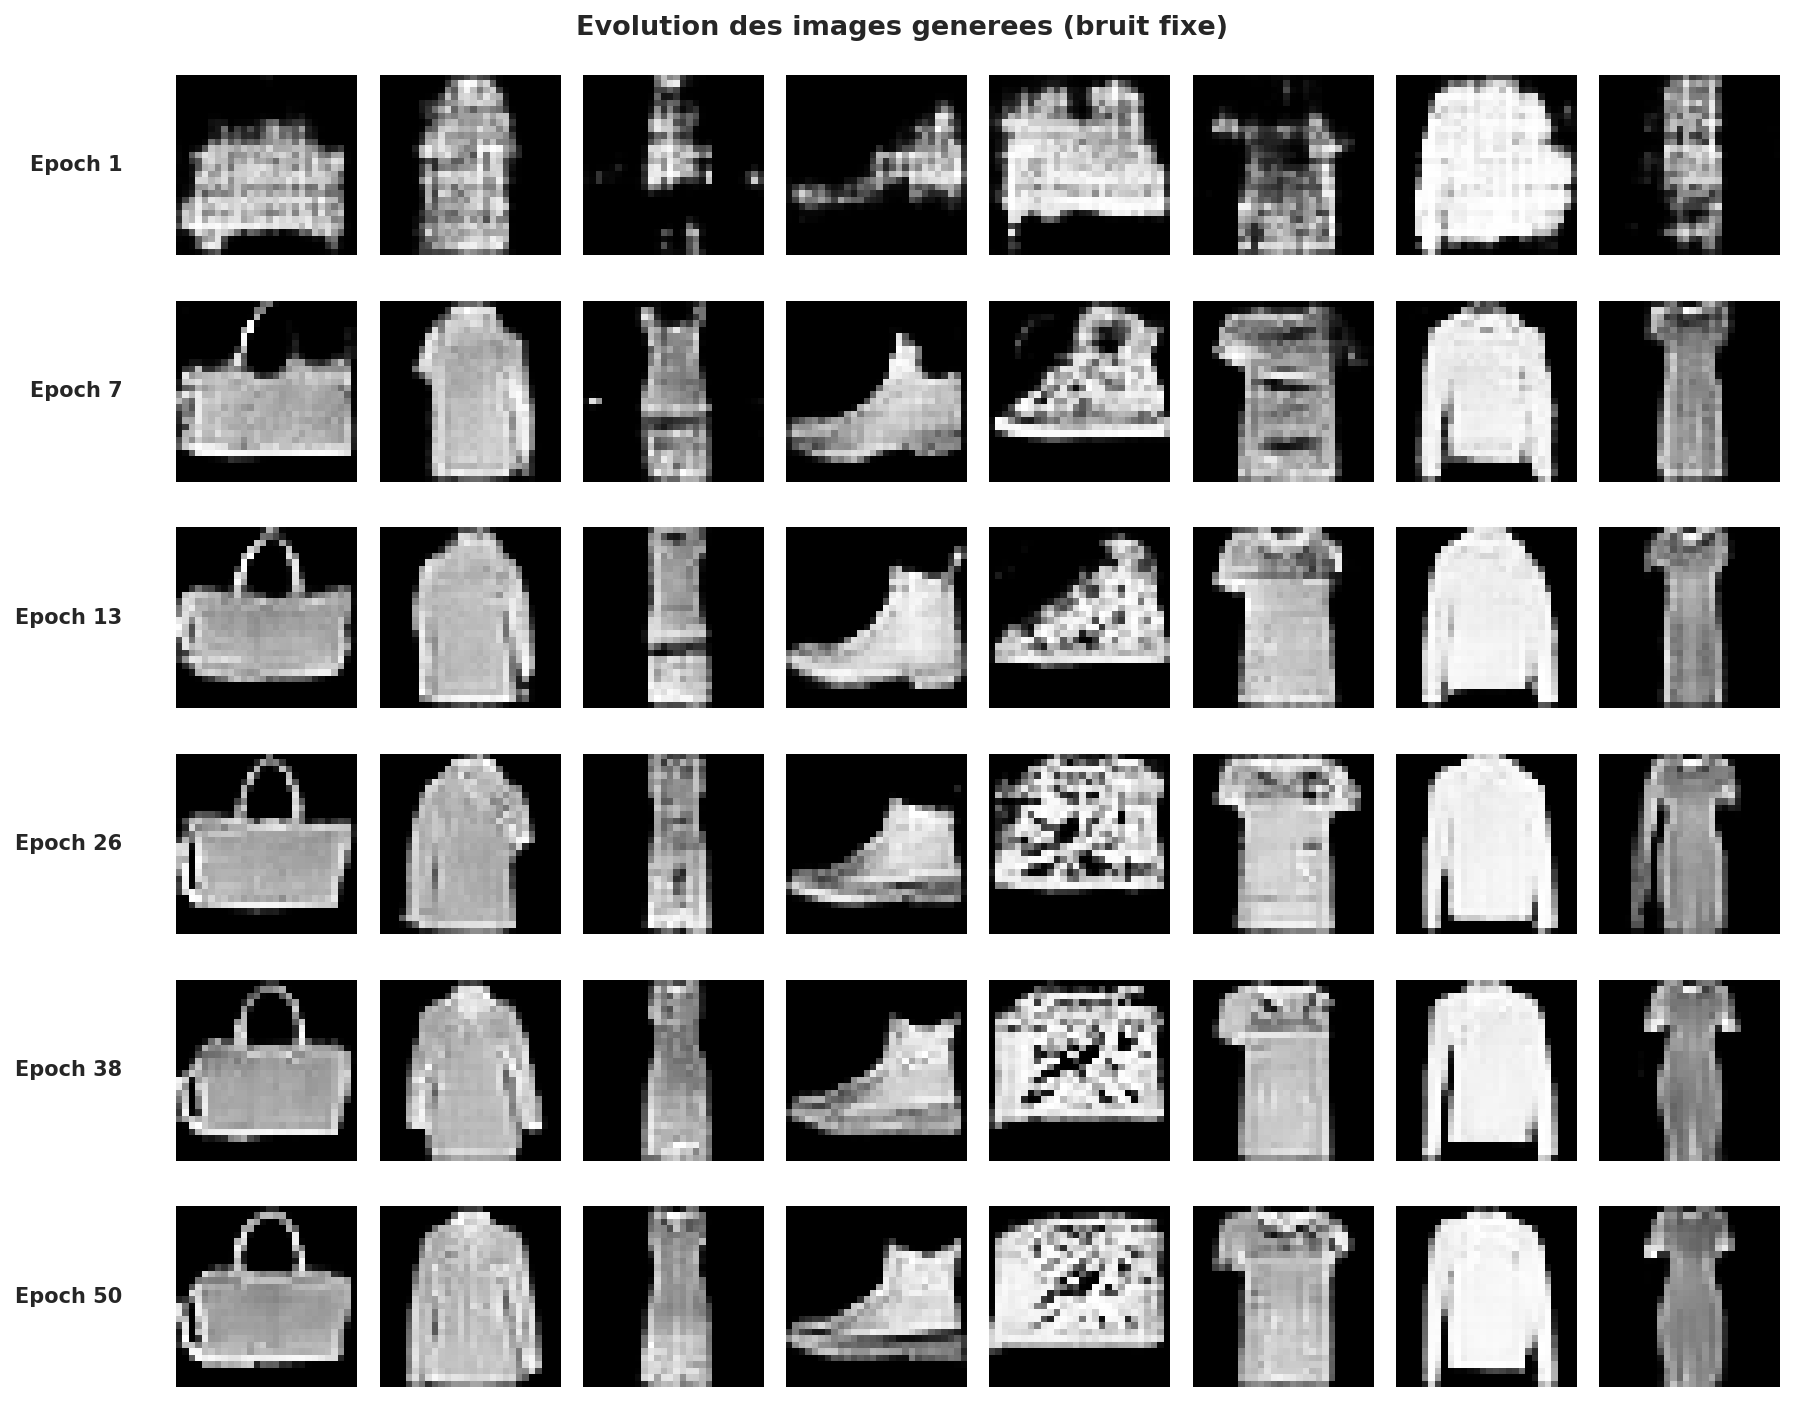
\includegraphics[width=\linewidth]{04_gan_evolution.png}
    \caption{Evolution du generateur a partir d'un bruit fixe sur 6 epochs reparties. Seul le generateur change d'une ligne a l'autre.}
    \label{fig:gan-evolution}
\end{figure}

La figure~\ref{fig:gan-evolution} montre la convergence du generateur. Des l'epoch 1, les sorties presentent les axes spatiaux corrects (silhouettes globales esquissees), meme si elles restent floues. A l'epoch 7, sept colonnes sur huit affichent un objet identifiable (sac, pull, robe, bottine, sneaker, t-shirt). Entre les epochs 13 et 50, l'amelioration se concentre sur les bords et le contraste : silhouette plus nette du sac, structure du col du pull mieux dessinee. \textbf{Le plafond qualitatif est atteint relativement tot}, ce qui est attendu pour un DCGAN sur un dataset aussi simple.

La cinquieme colonne illustre une pathologie locale : ce point latent precis se fige progressivement sur un motif de haute frequence sans semantique reconnaissable. Le generateur n'a pas reussi a y placer une classe valide ; il a appris a y placer une texture damier qui, statistiquement, trompe le discriminateur. C'est un cas typique de \emph{mode failure} ponctuel, par opposition au mode collapse global.

\begin{figure}[h]
    \centering
    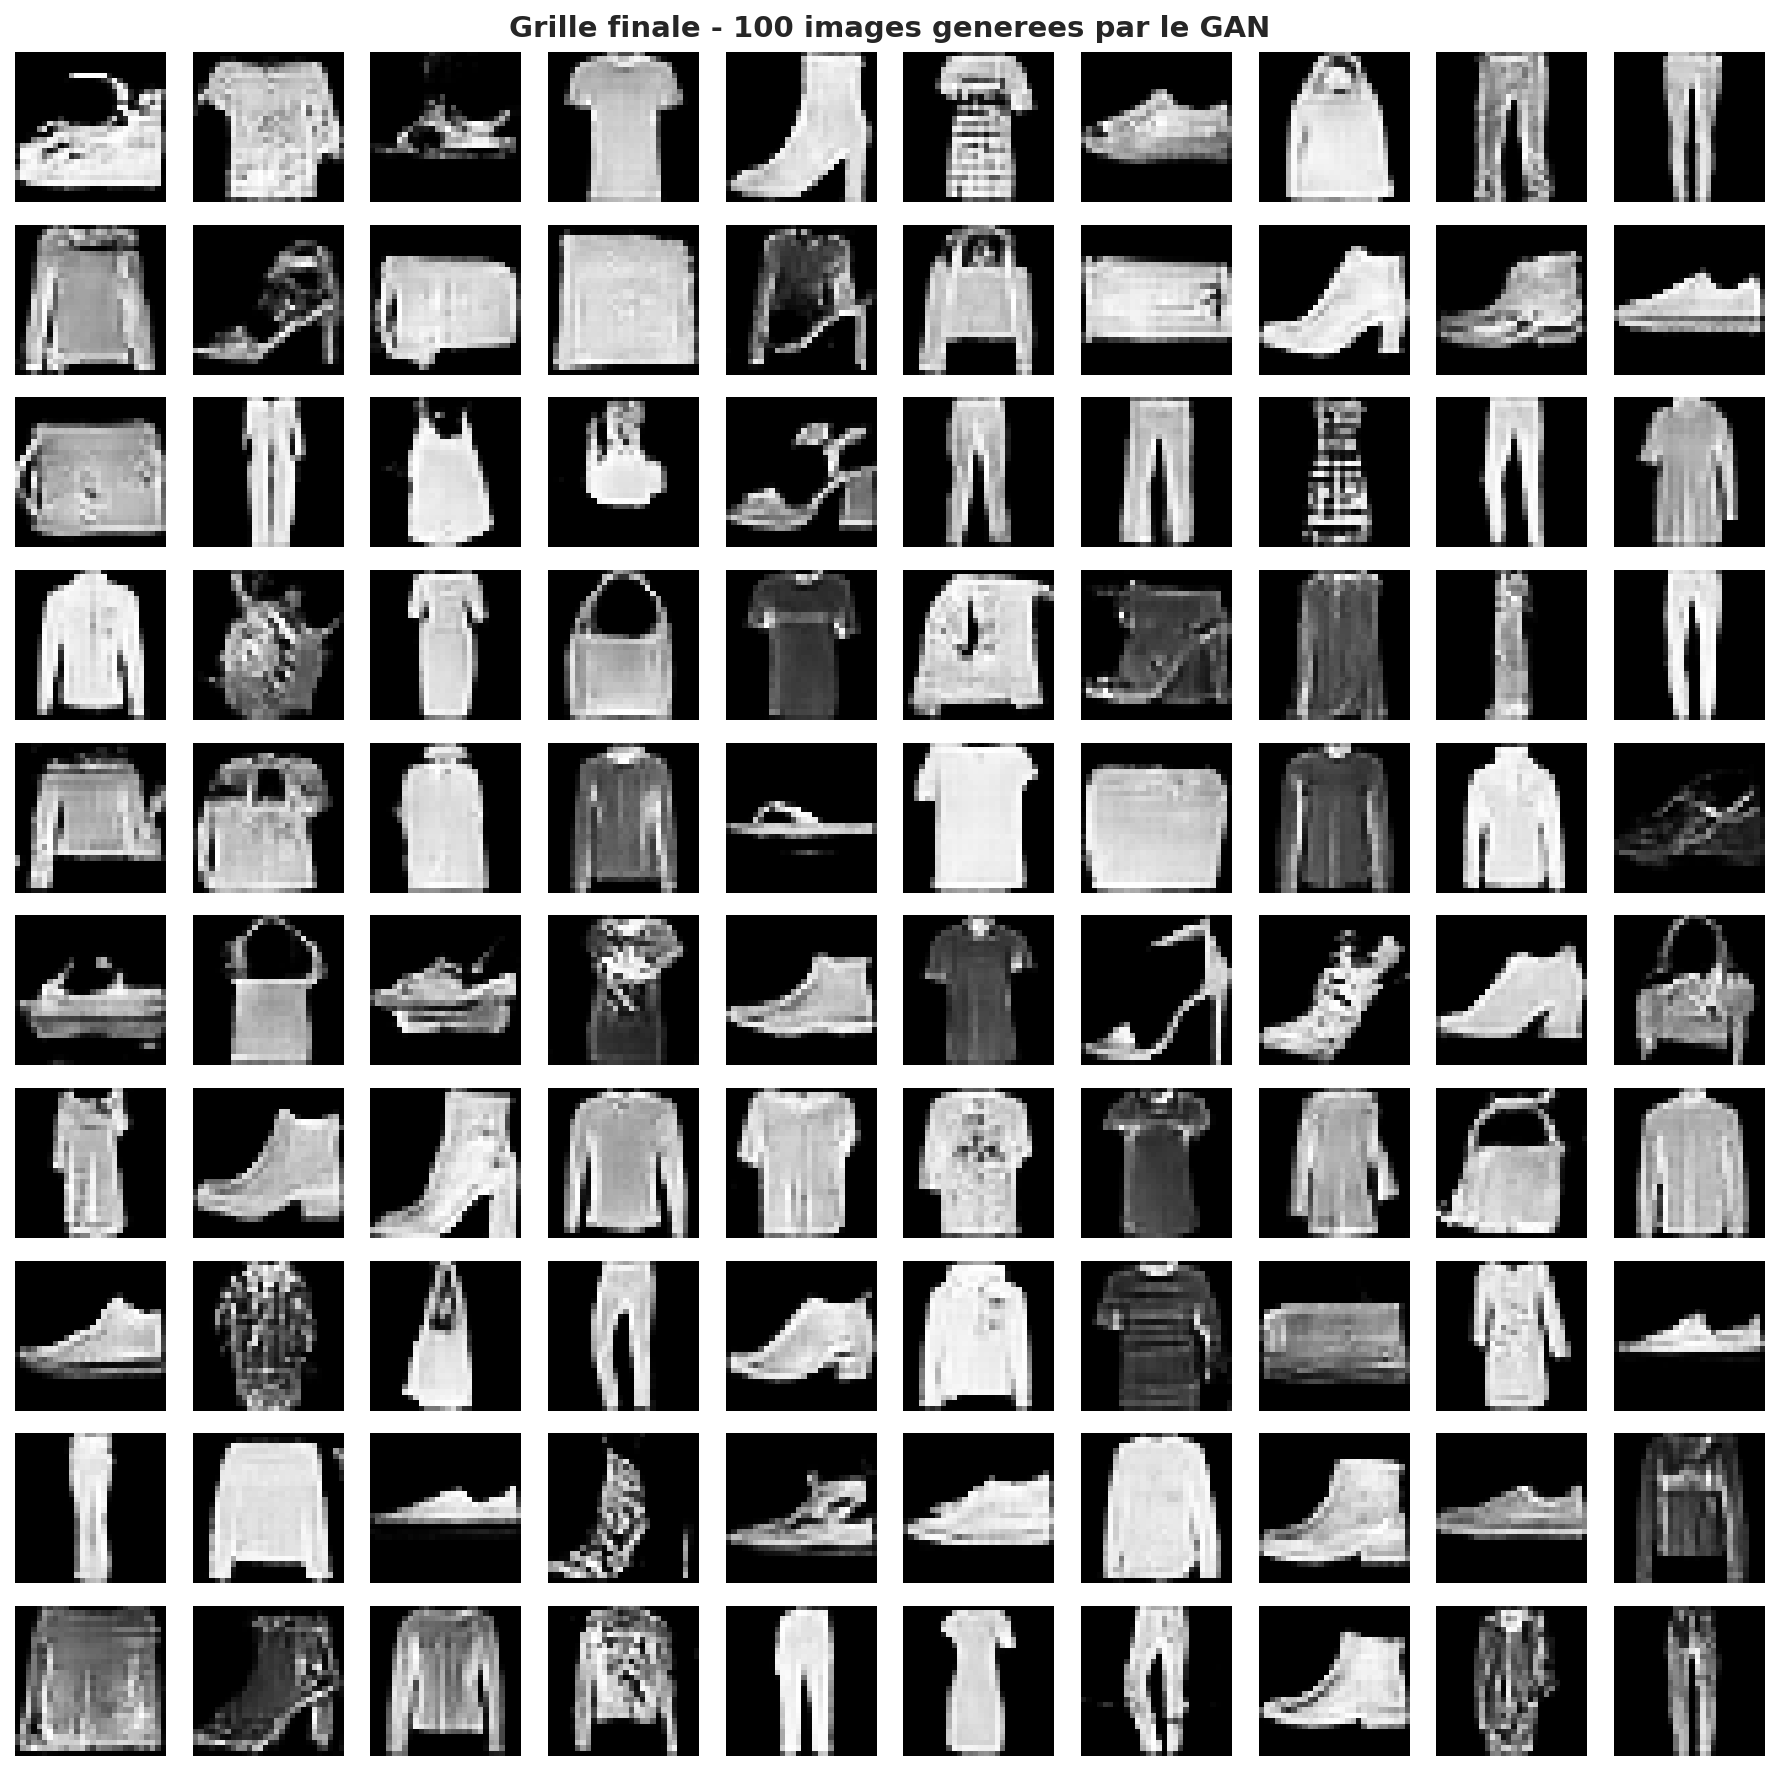
\includegraphics[width=0.85\linewidth]{05_gan_final_grid_100.png}
    \caption{Grille finale : 100 images independantes generees apres entrainement.}
    \label{fig:gan-grid}
\end{figure}

La grille de 100 images (figure~\ref{fig:gan-grid}) confirme \textbf{l'absence de mode collapse global} : on identifie des sacs, des pantalons, des bottines de hauteurs variables, des sneakers, des chaussures a talon, des hauts et des robes. La diversite est reelle mais inferieure a celle du dataset original :

\begin{itemize}
    \item sur-representation visuelle des classes structurellement simples (Pantalon, Sac) ;
    \item sous-representation des chaussures detaillees (Sandale en particulier) ;
    \item plusieurs cases contiennent des silhouettes hybrides T-shirt/Chemise/Pull non identifiables, conformes a la difficulte inter-classes anticipee section~\ref{sec:dataset} ;
    \item quelques cases tres claires sans structure precise, traduisant des zones latentes mal couvertes.
\end{itemize}

\subsection{Bilan sur le GAN}

Le DCGAN entraine 50 epochs sur Fashion-MNIST produit des images globalement realistes, avec une diversite correcte mais imparfaite et des defauts caracteristiques attendus : flou sur les bords (artefacts des \texttt{ConvTranspose2d} a stride 2), asymetries, hybridations entre classes proches. La convergence visuelle est rapide ($\approx$ 7 epochs) et la qualite plafonne ensuite. Les pathologies observees (mode failure local, derive de la \texttt{G\_loss}) s'expliquent par les choix d'architecture et la dynamique adversariale, et constituent le materiau de comparaison avec les modeles de diffusion traites dans la partie suivante.

% Bibliographie a fusionner avec celle du rapport general.
% @inproceedings{xiao2017fashion,
%   title={Fashion-MNIST: a Novel Image Dataset for Benchmarking Machine Learning Algorithms},
%   author={Xiao, Han and Rasul, Kashif and Vollgraf, Roland},
%   booktitle={arXiv:1708.07747},
%   year={2017}
% }
% @inproceedings{radford2015dcgan,
%   title={Unsupervised Representation Learning with Deep Convolutional Generative Adversarial Networks},
%   author={Radford, Alec and Metz, Luke and Chintala, Soumith},
%   booktitle={ICLR},
%   year={2016}
% }
